\documentclass[10pt]{scrartcl}

\usepackage{graphicx}
\usepackage{subcaption} 
\usepackage{float}
\usepackage{nameref}
\usepackage{color,soul}

\title{Scientific Experimentation and Evaluation\\
		\small{Assignment 3}}
\author{Chaitanya Hebbal\\
		Jos\'e Carlos Mayoral Ba\~nos}

\begin{document}
	\maketitle
\section*{Task Description}

Our \textbf{task} is defined as: \textit{Constructing a LEGO NxT differential drive robot and manually measure the observable pose variation for three different velocity motions}. The goal of this experiment is to observe the variation on the manual measured poses and look at the error distributions.

%In order to achieved the goal, there are some constraints that must be taken into account:

%\begin{itemize}
%	\item The Device Under Test is a LEGO NxT robot.
%	\item DifferentialPilot library for motion behaviour.
%	\item Manual measurement comes out with additional error provided by the person who makes them.
%	\item The time of every movement must be constant.
%	\item There is not a true value to compare with, this must be obtained from the repetitions of the experiment.
%\end{itemize}

The layout of this experiment consists on:
\begin{enumerate}
%	\item DifferentialPilot library for motion behaviour.
%	\item Manual measurement comes out with additional error provided by the person who makes them.
%	\item The time of every movement must be constant.
%	\item There is not a true value to compare with, this must be obtained from the repetitions of the experiment.
	\item Five different curves movements are going to be measured: Straight line and 4 arcs (2 left and 2 right).
	\item The Device Under Test is a LEGO NxT robot.
	\item A third-part library for the software is previously defined.
\end{enumerate}

Plan for the experiment is given below:

\begin{enumerate}
	\item Define the measurement method (see below).
	\item Code a good program which takes into consideration the provided restrictions.
	\item Define the curves that must be done according to pre-defined library.
	\item Store the information of the final poses.
	\item Repeat twenty times every curve measurement.
	\item Compute the information to get the error gaussian distribution.
\end{enumerate}

\section*{Experiment setup}

\subsection*{Device Under Test}

The Device Under Test is a LEGO NxT robot, shown at figure \ref{fig:1}.

\begin{figure}[h!]
\centering
\caption{LEGO Nxt Robot}
\label{fig:1}
  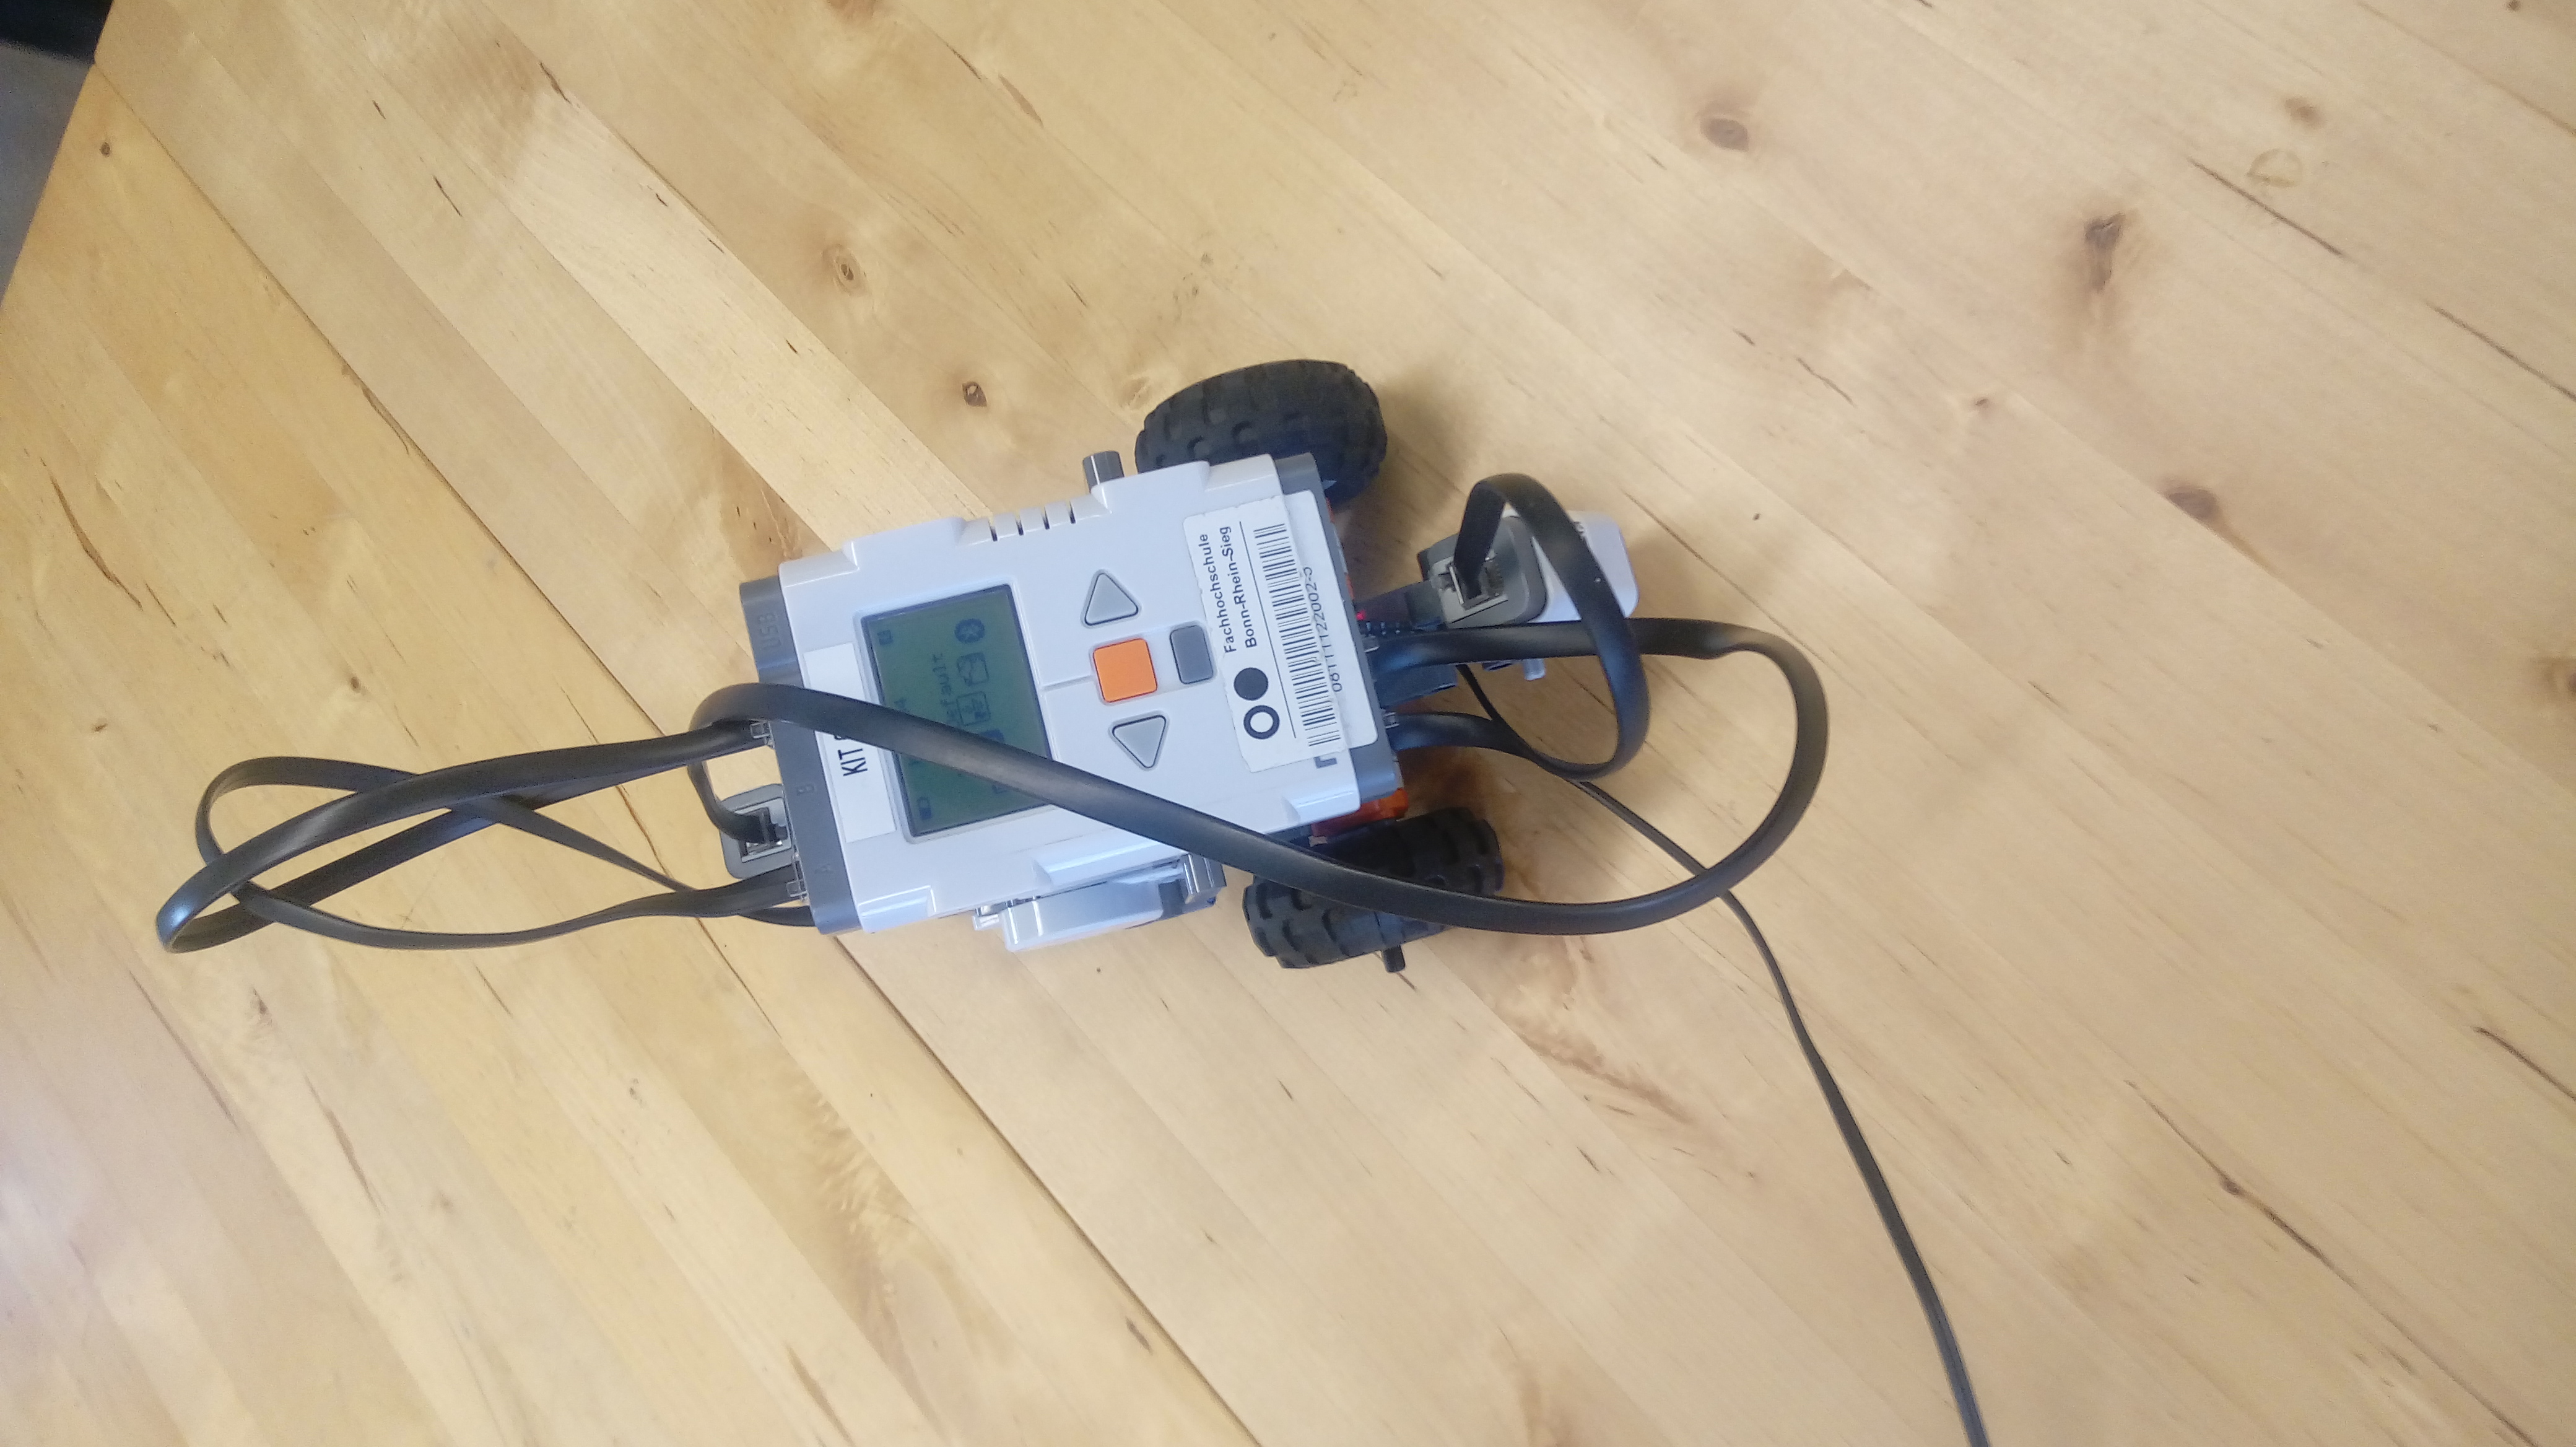
\includegraphics[width=0.49\textwidth]{images/robot_1}
  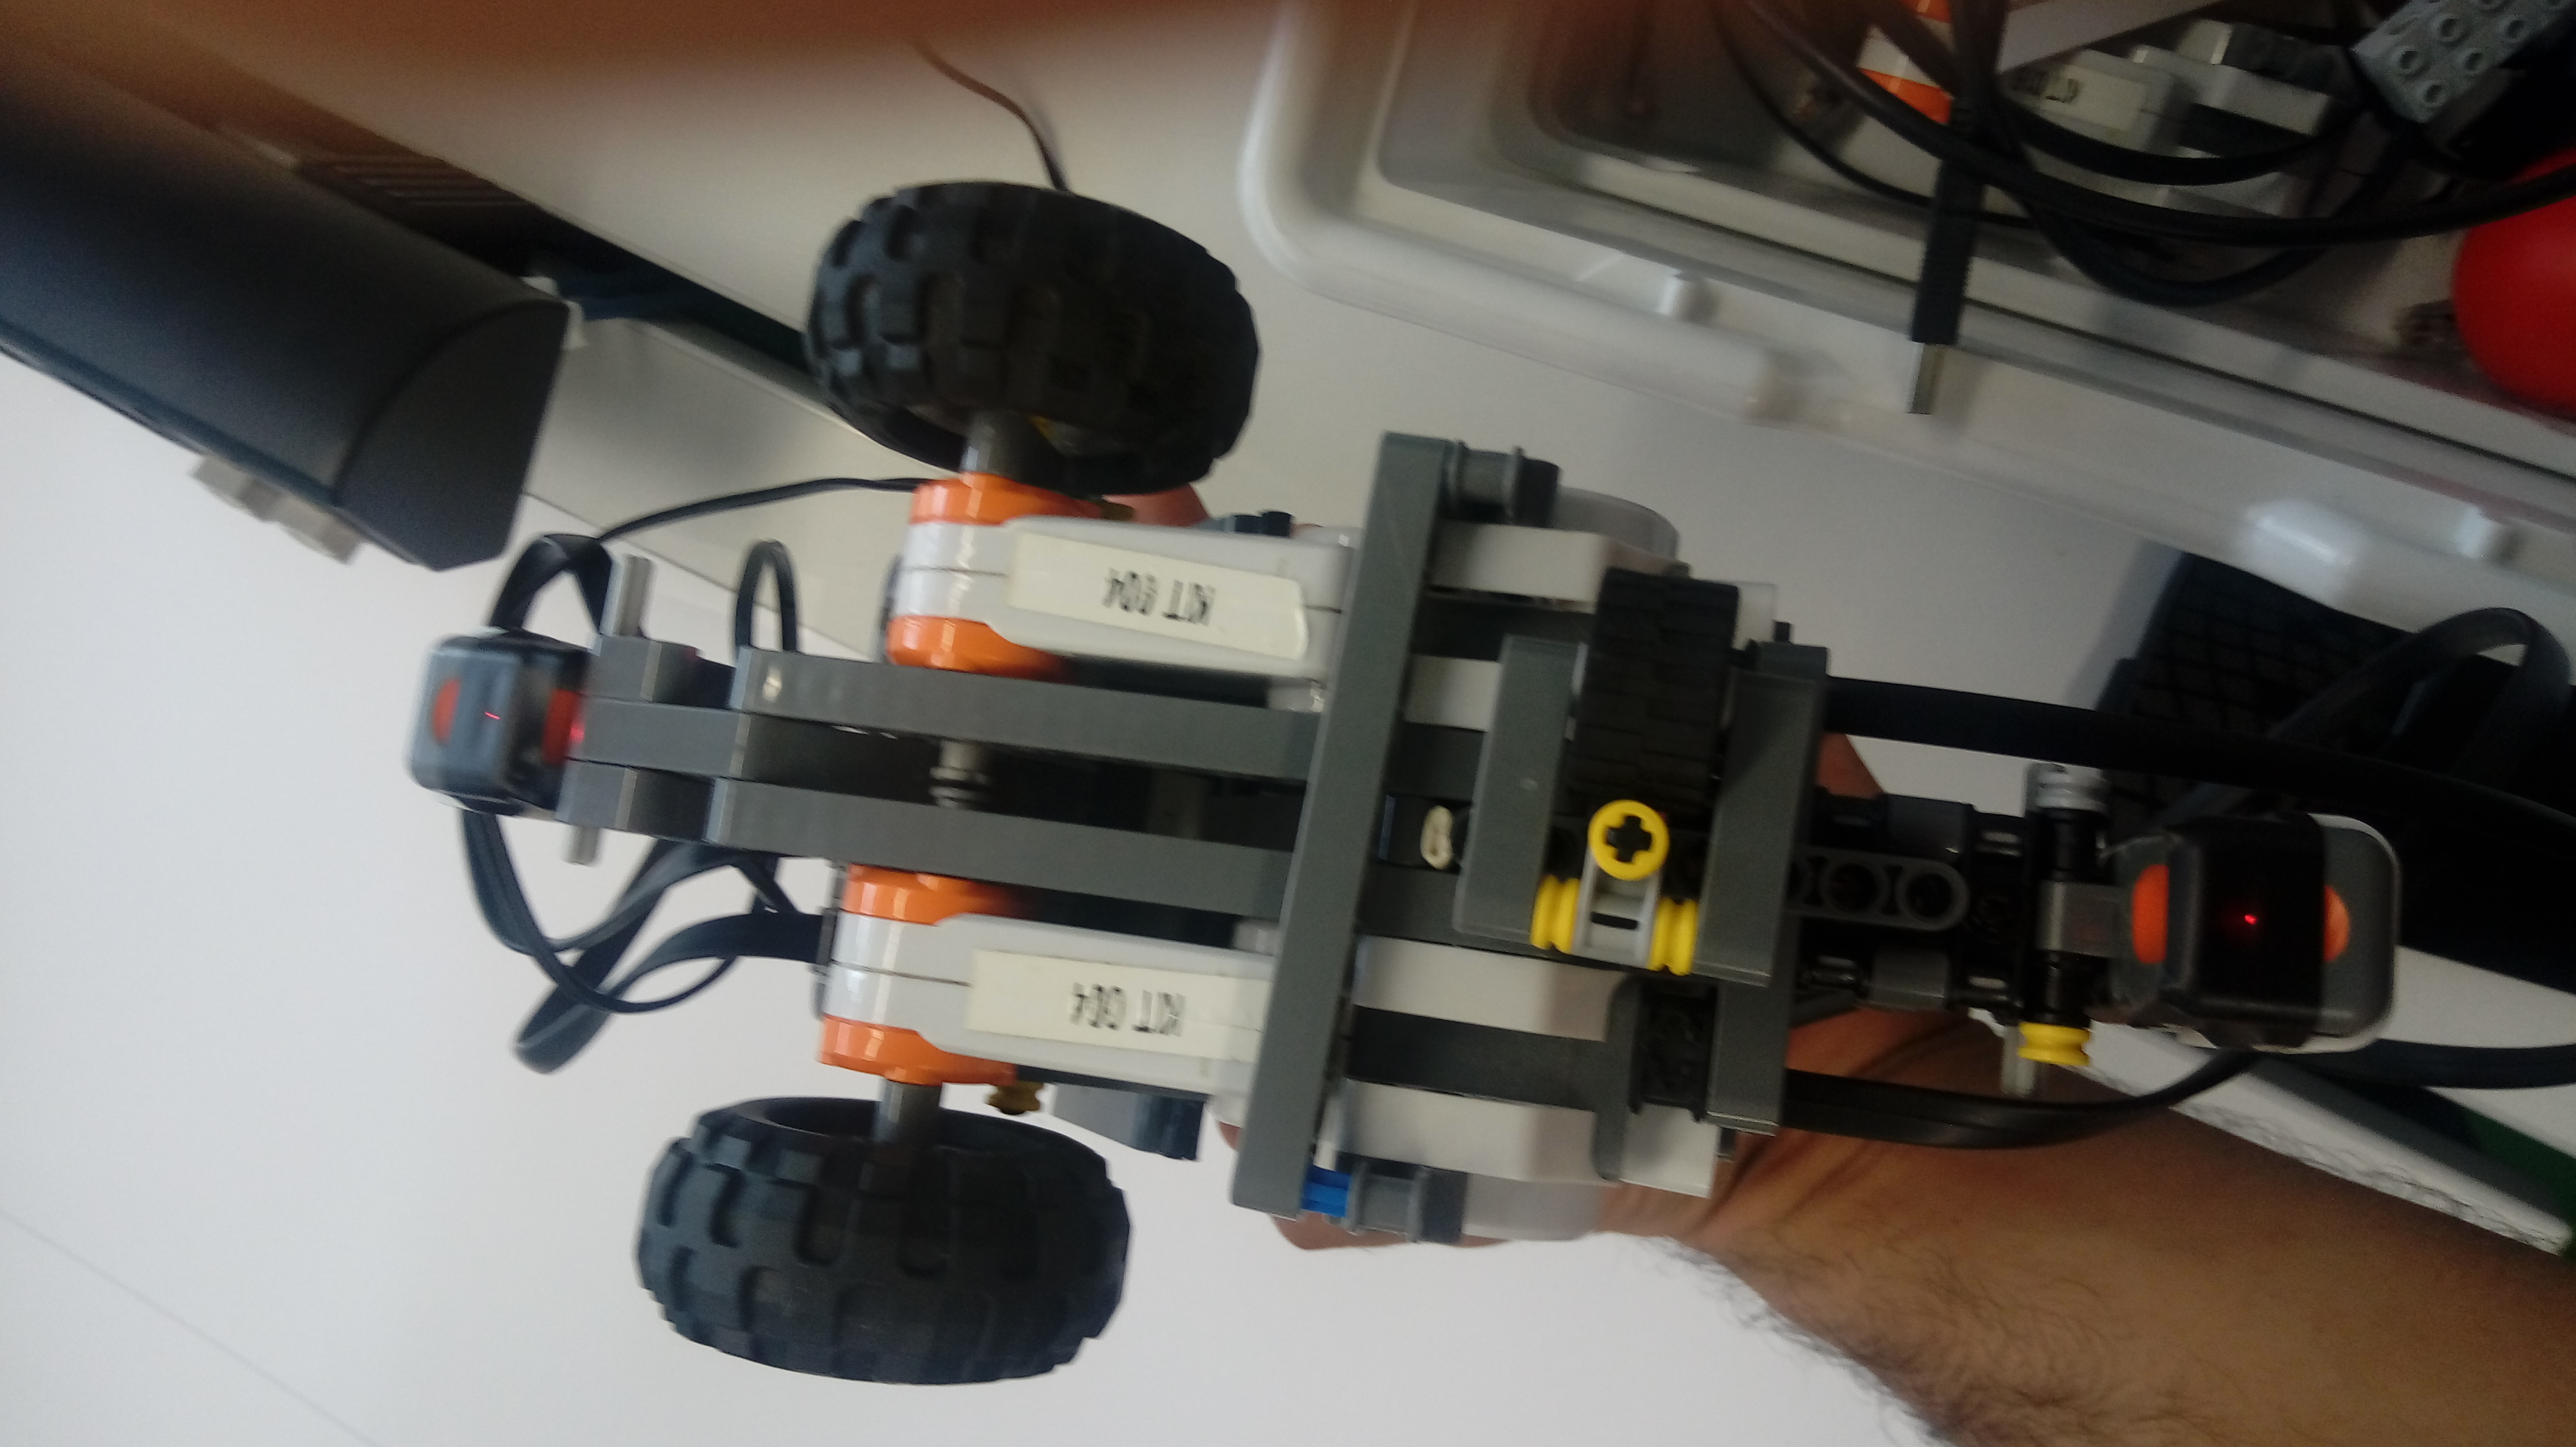
\includegraphics[width=0.49\textwidth]{images/robot_2}
\end{figure}

\subsection*{Measured Value}
The polar coordinate of the robot (distance to origin, and angle $ \theta $).

\subsection*{Measurement System}

The measurement value (final pose) is acquired by a LEGO NxT robot which uses the libraries provided by leJOS framework for motion and a large cardboard sheet, light sensor and geometric representation to acquire data. 

\subsection*{Measuring Method}

To accomplish the task we have defined the experiment as explained in the picture.\\

\begin{figure}[h!]
\caption{Experiment Description}
\label{fig:2}
\centering
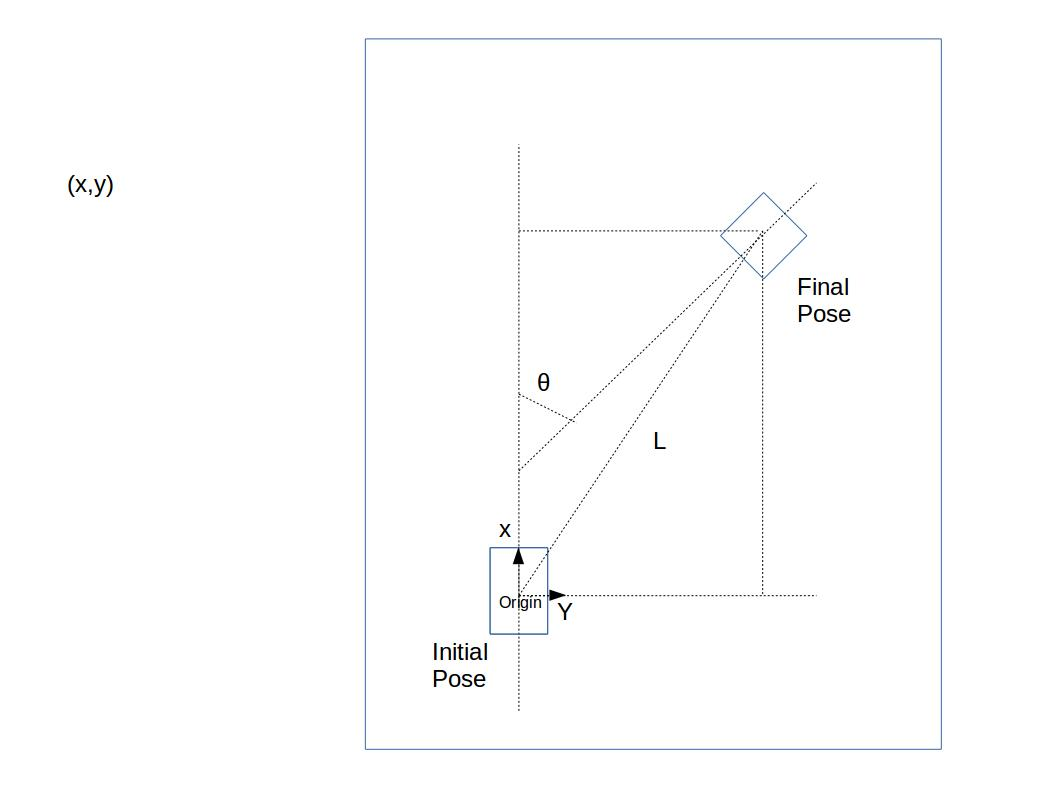
\includegraphics[trim=300 0 0 0, clip,scale=0.35]{images/exp1}
\end{figure}

The method description of image \ref{fig:2} is:
\begin{itemize}
	%\item One LEGO structure will set the robot at initial position so the initial position will be constant.
	\item A cardboard is used to mark the points of all the experiment.
	\item Two light sensors are used to mark the points in order to get the pose of the robot.
	\item Using LEGO light sensors initial pose is marked on the cardboard.
	\item A perpendicular axis which connects two original points is drawn as a reference.
	\item The origin is located between wheels so there distance from a sensor to the center must be measured. 
	\item After the robot stops, a projection of the line is drawn between the two measured points pointed by the sensors.
	\item The angle will be measured between the reference axis and the projected line.
	\item From the final marks, the new center is calculating extracting distance from initial marker to center along the projected line.
	\item Linear distance comes from the distance between measured center the and origin.
	\item For every repetition the initial pose must fit the original pose markers.	
	\item After 5 repetitions, erase marks in order to get better measurements.
\end{itemize}

The Measurement facilities include:

\begin{itemize}
	\item One cardboard.
	\item Two light sensors.
	\item A pen.
	\item A protractor.
	\item A rule.
\end{itemize}

The used light markers use is shown at image \ref{fig:3}.

\begin{figure}[h!]
\centering
\caption{LEGO Nxt Robot Light Markers}
\label{fig:3}
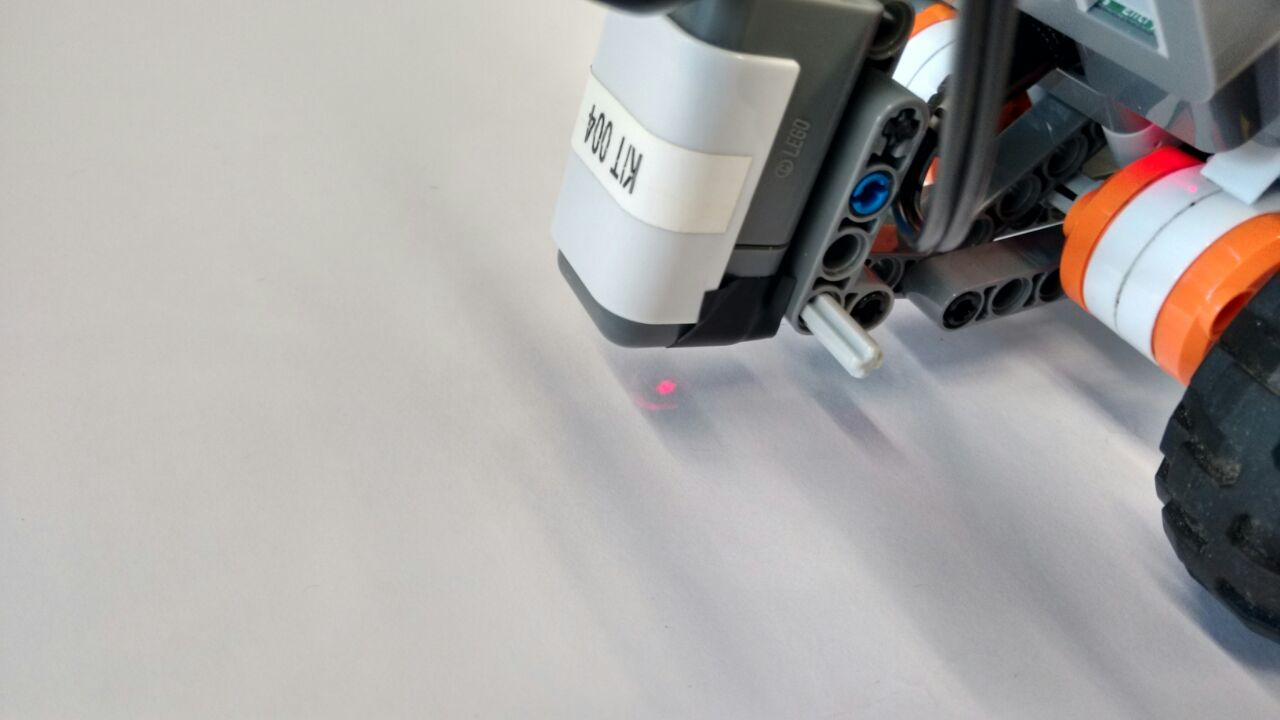
\includegraphics[width=0.49\textwidth ]{images/marker_1}
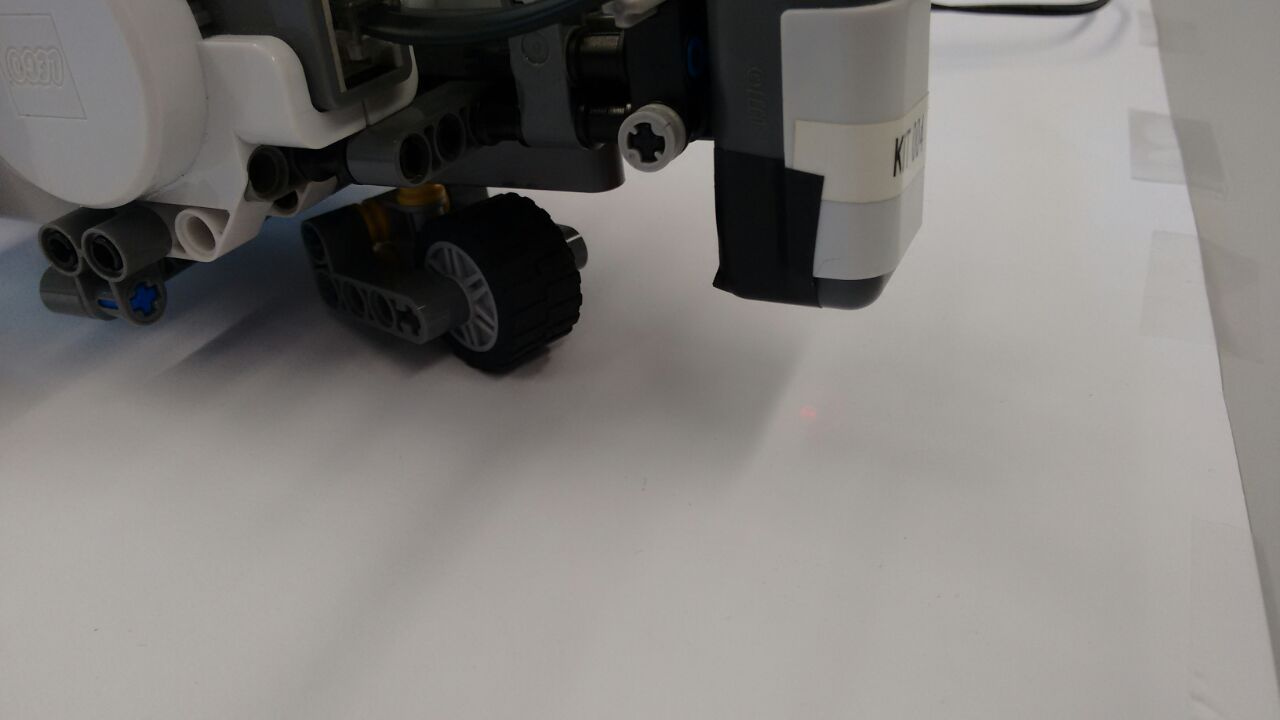
\includegraphics[width=0.49\textwidth]{images/marker_2}
\end{figure}


\subsection*{What difficulties are expected?}

In order to accomplish the current task, we found the following constraints:

\begin{itemize}
	\item The manual measurement will add errors to the measurement result.
	\item The precision of the instruments will affect the gaussian distribution.
\end{itemize}

\section*{Experimental Observations}

An example of the measurement process can be seen at figure \ref{fig:4}, this example comes from the straight line experiment.

\begin{figure}[h!]
\centering
\caption{LEGO Nxt Robot Light Markers}
\label{fig:4}
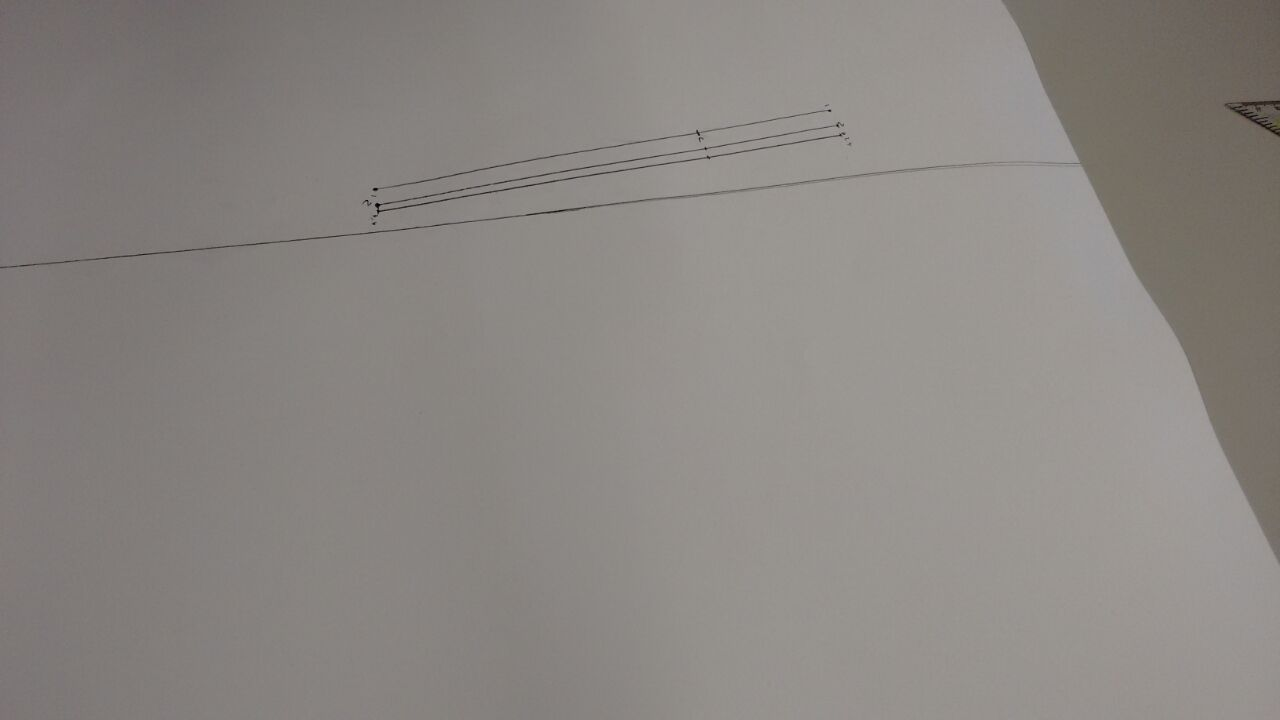
\includegraphics[trim={200 400 300 50},clip,scale=0.4]{images/measurements}
\end{figure}

The right motor seems to be steeper as the left one, i.e. the straight line deviates to left (image \ref{fig:5}). This effect is also observable at the other curves. The experiment trim shows us the last five measurements that were taken.

\begin{figure}[h!]
\centering
\caption{Experiments print}
\label{fig:5}
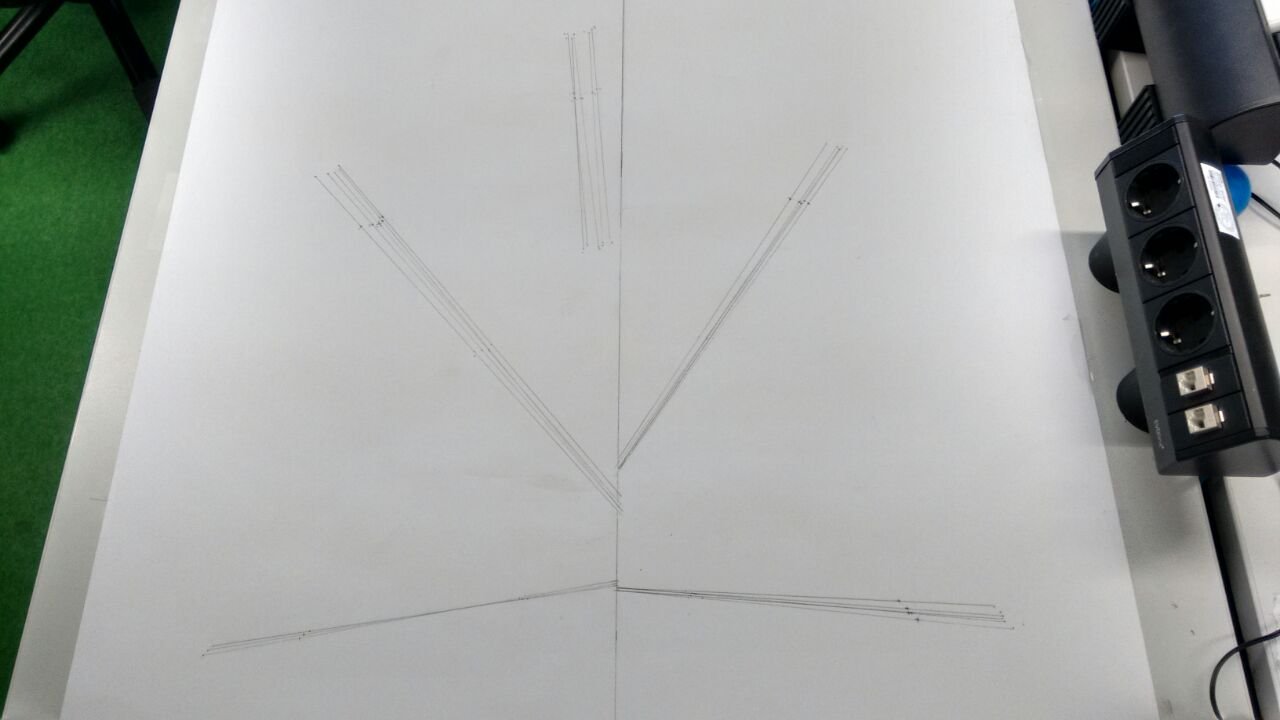
\includegraphics[scale=0.3,trim={170 0 240 0},clip]{images/print}
\end{figure}

\subsection*{Precision and Accuracy}

The precision of the experiment relies on the precision of the measurement facilities:
\begin{itemize}
	\item For Distance Measurement: the rule was used which precision is 1 mm.
	\item For Angle Measurement: the protractor was used which precision is 1$^{\circ}$.
\end{itemize}

\newpage
\subsection*{Parameters used to drive the robot}

\begin{table}[ht!]
\centering
\caption{Parameters Used}
\label{tab:1}
\begin{tabular}{|c|c|c|c|c|} \hline
 				& Arc radius& Angle & Distance & Track Width \\ \hline
Steep left arc  & 20        & 90    &          & 12 \\ \hline
Steep right arc & 20        & 90    &          & 12 \\ \hline
Soft left arc   &           & 40    & 55       & 12 \\ \hline
Soft right arc  &           & 40    & 55       & 12 \\ \hline
Straight        & 40        & 90    &          & 12 \\ \hline
 
\end{tabular}
\end{table}

\subsection*{Experiments Results}

The experiments lead to the results provided at the attached file $first\_see\_data\_.ods$. In them, we can see that the  protractor precision is not enough for this experiment due to the fact that many measurements fell somewhere between the scale so the measurement were round to the closer value. This round affects the accuracy of the experiment.

In addition of this, the design measurement system lacks of information in order to calculate the pose angle because with the distance from origin to robot final center these angle cannot be calculated. Therefore, the accuracy of the angle cannot be improved. \\

As consequence, a new measurement system is was designed to improve these results. The next section will provided the new measurement system.

\subsection*{Improved Measuring Method}

For this new measuring method, the already provided robot structure at figure \ref{fig:3} and parameters at table \ref{tab:1} remain with no changes. In other words, the differential drive platform and light sensors are also considers for this method. However the number of repetitions were increased from twenty to forty.\\

For the new method, the next measurement facilities will be needed:

\begin{itemize}
	\item One cardboard.
	\item Two light sensors.
	\item 10 pens of different color.
	\item A rule.
\end{itemize}


\begin{figure}[h!]
\centering
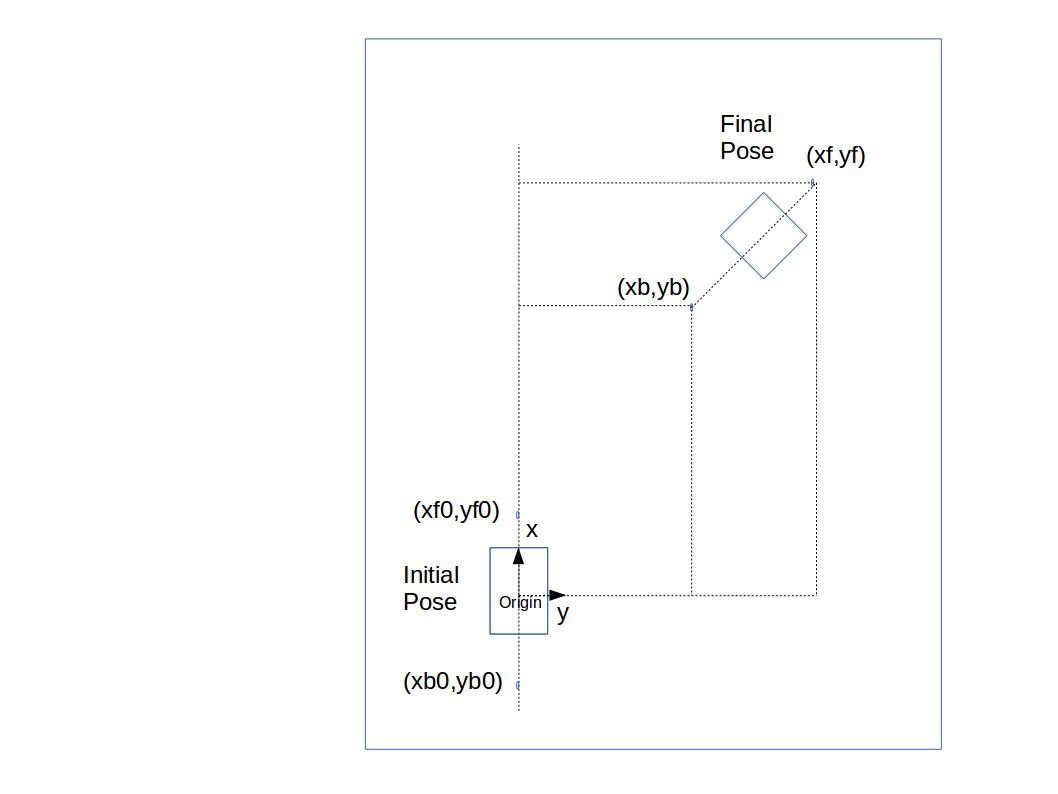
\includegraphics[trim=200 0 0 0, scale=0.35]{images/exp2}
\caption{Improved Experiment Description}
\label{fig:6}
\end{figure}

The modified method description of figure \ref{fig:6} is:
\begin{itemize}
	%\item One LEGO structure will set the robot at initial position so the initial position will be constant.
	\item A cardboard is used to mark the points of all the experiment.
	\item A world frame is drawn on the cardboard.	
	\item Two light sensors are used to mark the points in order to get the pose of the robot.
	\item Using LEGO light sensors initial pose is marked on the cardboard with a point (one for front light sensor and other for backward light sensor).
	\item The program is run in the robot.
	\item When the robot stops, a new set of points(x,y) for each sensor are marked using the rule on the cardboard with a pen of different color.
	\item For every repetition the robot should be aligned according to the original points in order to warranty that the start pose is the same.
	\item After 10 repetitions (each one with different color) the points are measured and in order to not confuse the next round the points will be marked with a different shape.
	\item Having 40 repetitions of one curve, a different curve must be measured. In total, there are 5 different curves (200 repetitions).
\end{itemize}

\subsection*{Experiment Settings}

A coordinate frame must be drawn at the cardboard (figure \ref{fig:7}) A line was drawn every 10 cm for each axis.

\begin{figure}[h!]
\centering
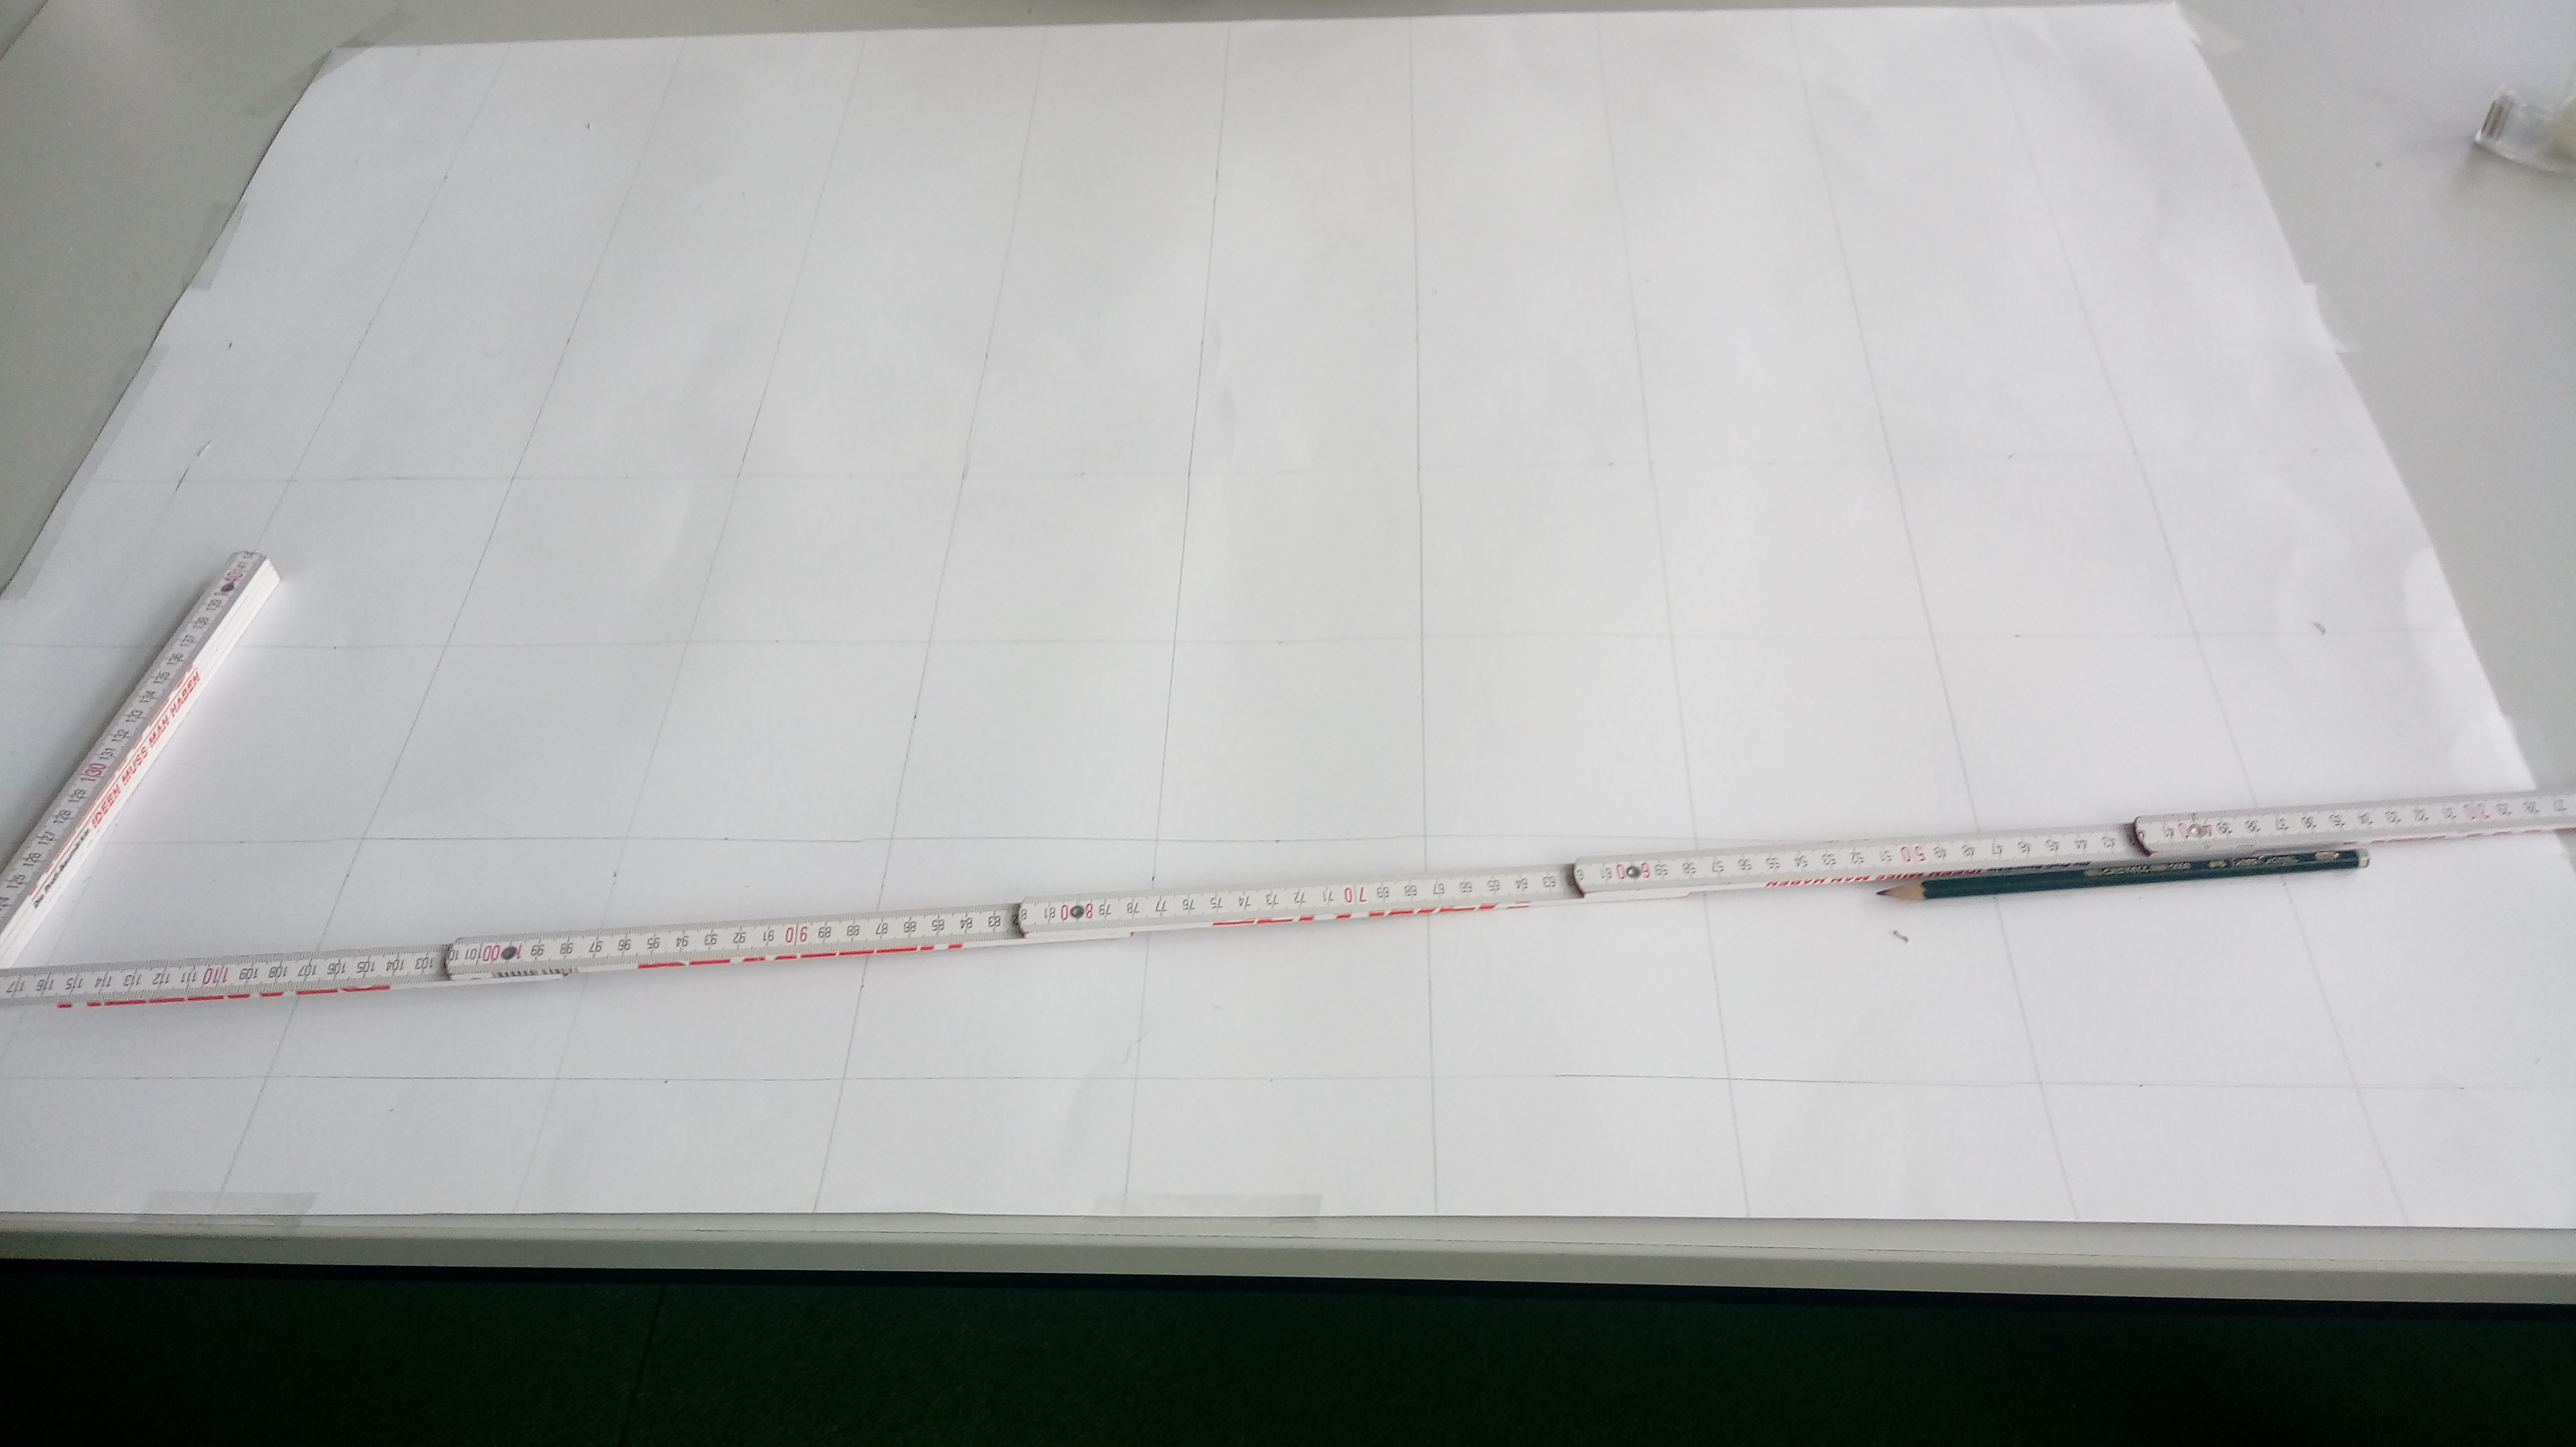
\includegraphics[trim=200 0 0 0, scale=0.10]{images/settings2}
\caption{Coordinates Frames Draw Process}
\label{fig:7}
\end{figure}

The complete grid is shown in the figure \ref{fig:8}.

\begin{figure}[h!]
\centering
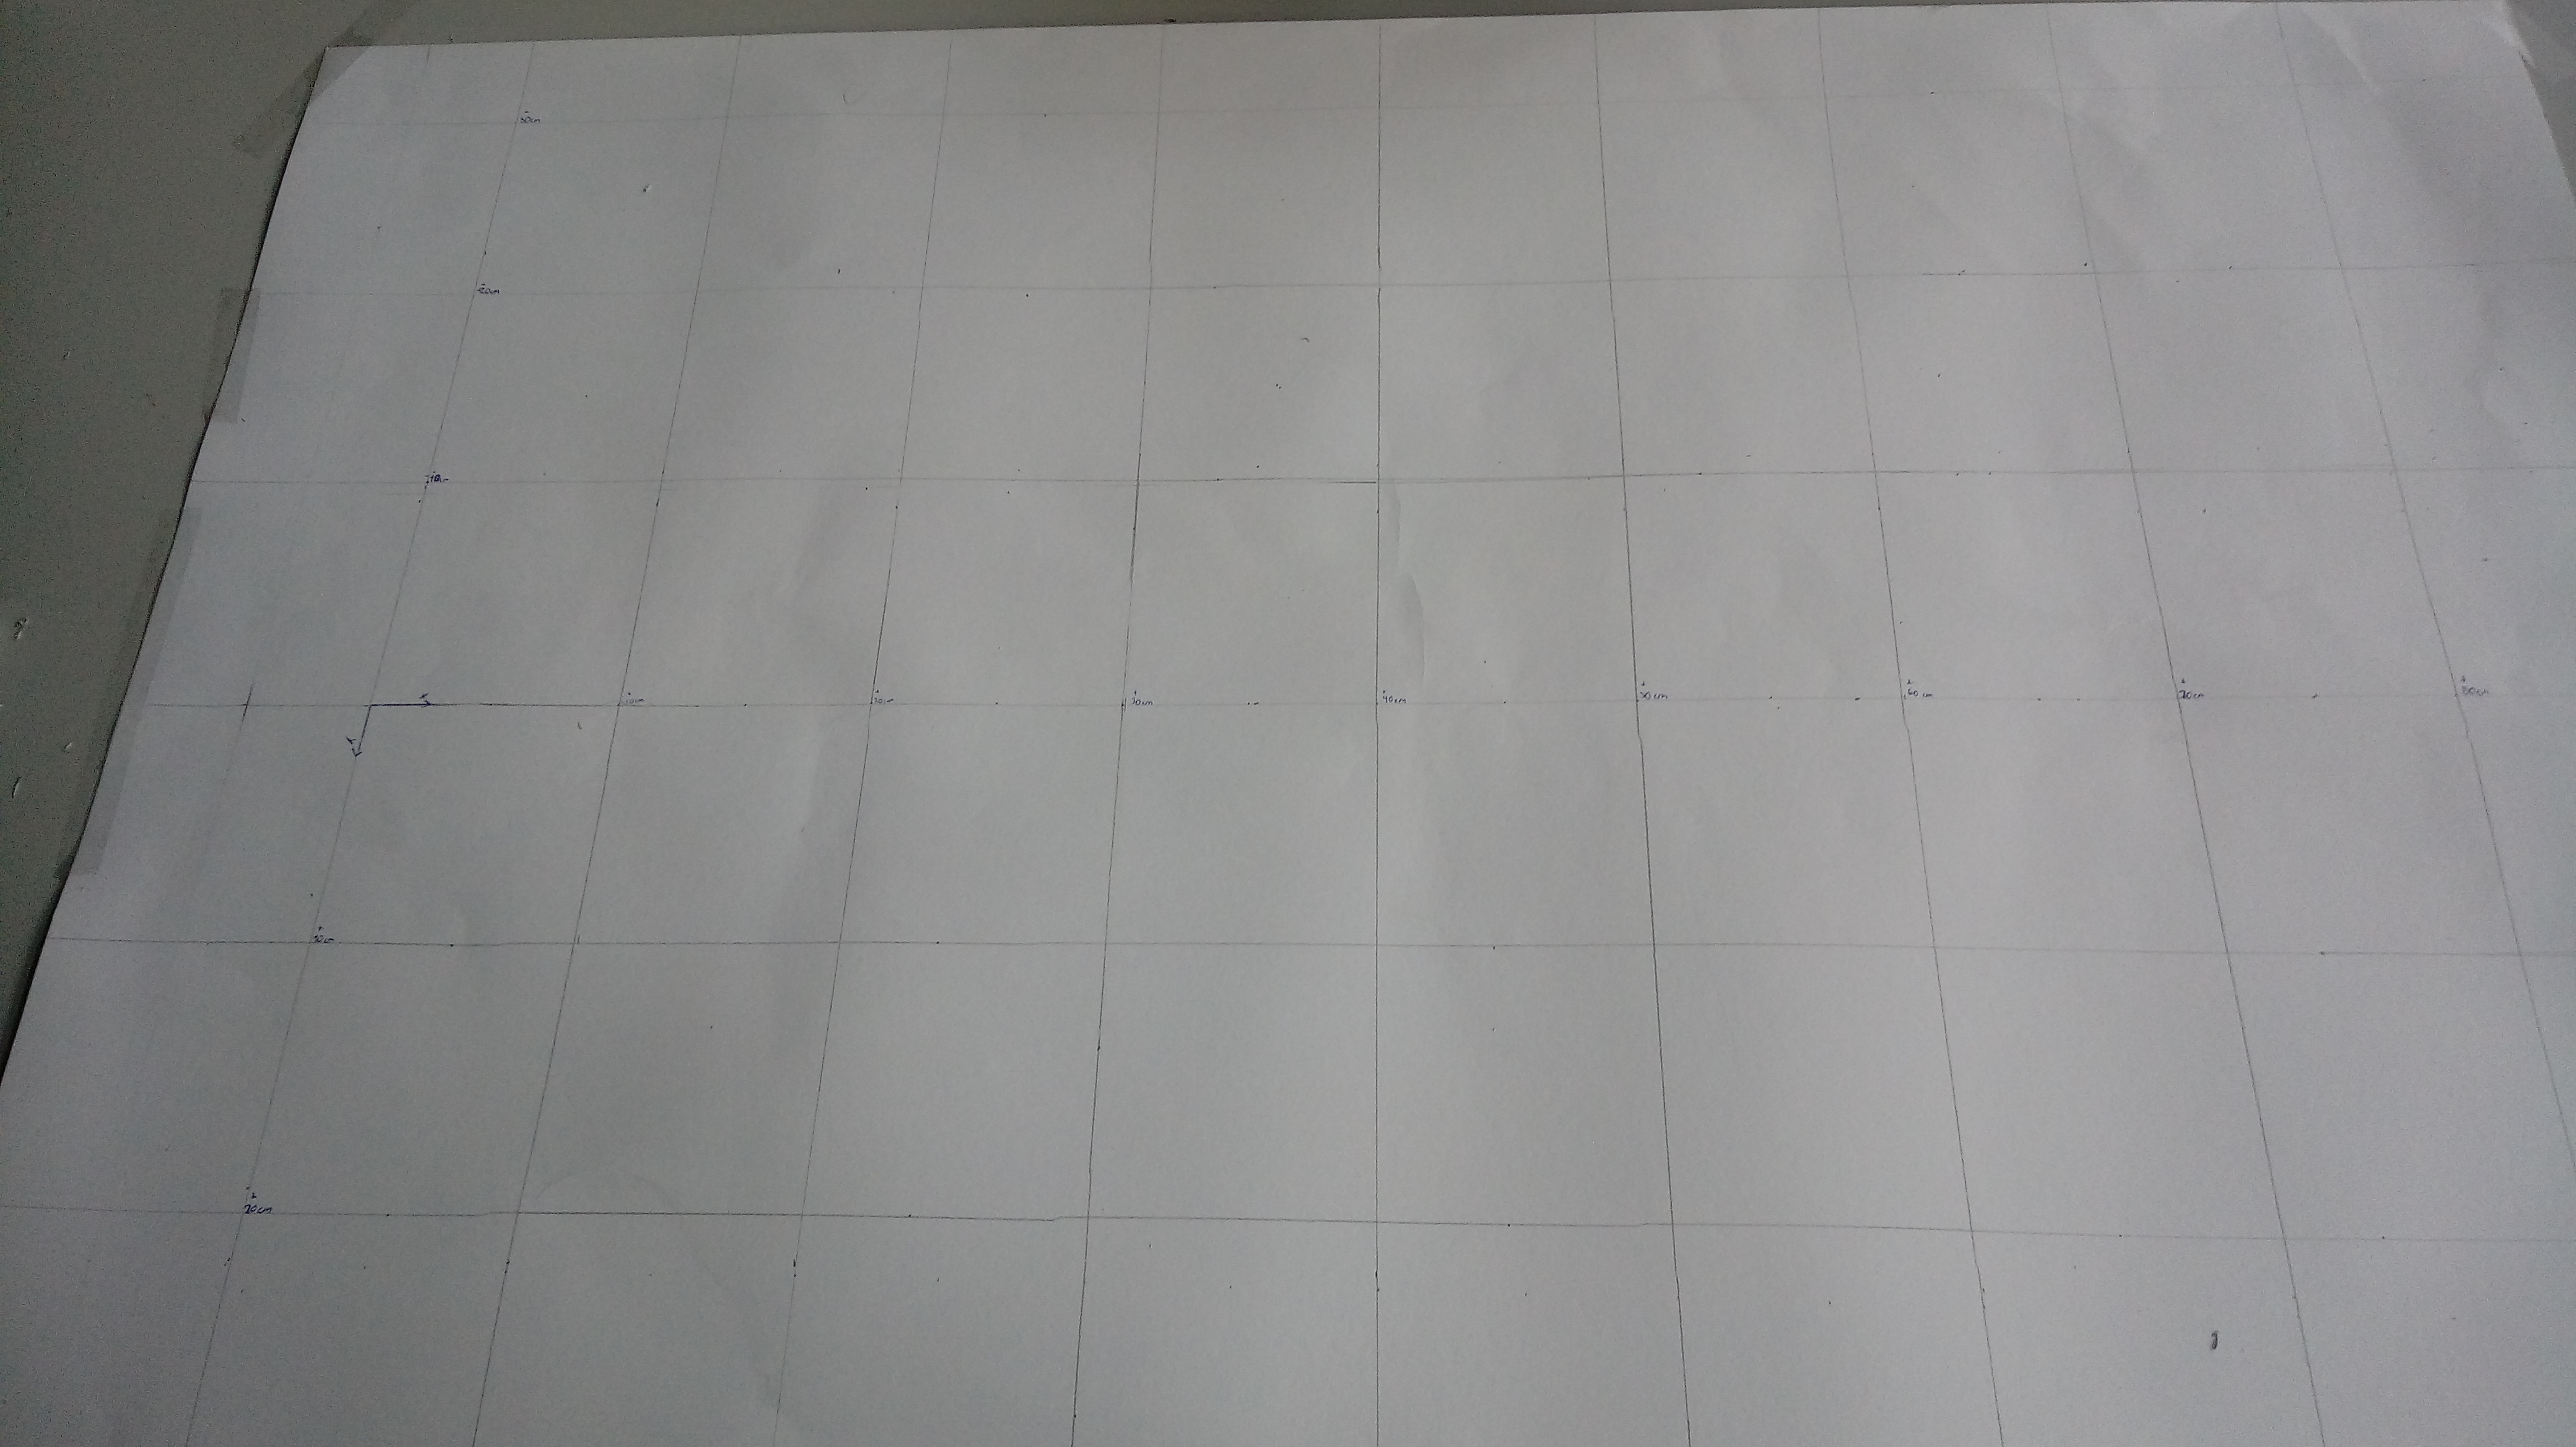
\includegraphics[trim=200 0 0 0, scale=0.10]{images/settings3}
\caption{Complete Coordinates frames}
\label{fig:8}
\end{figure}

A world origin frame was selected on the grid (shown at  figure \ref{fig:9}).

\begin{figure}[h!]
\centering
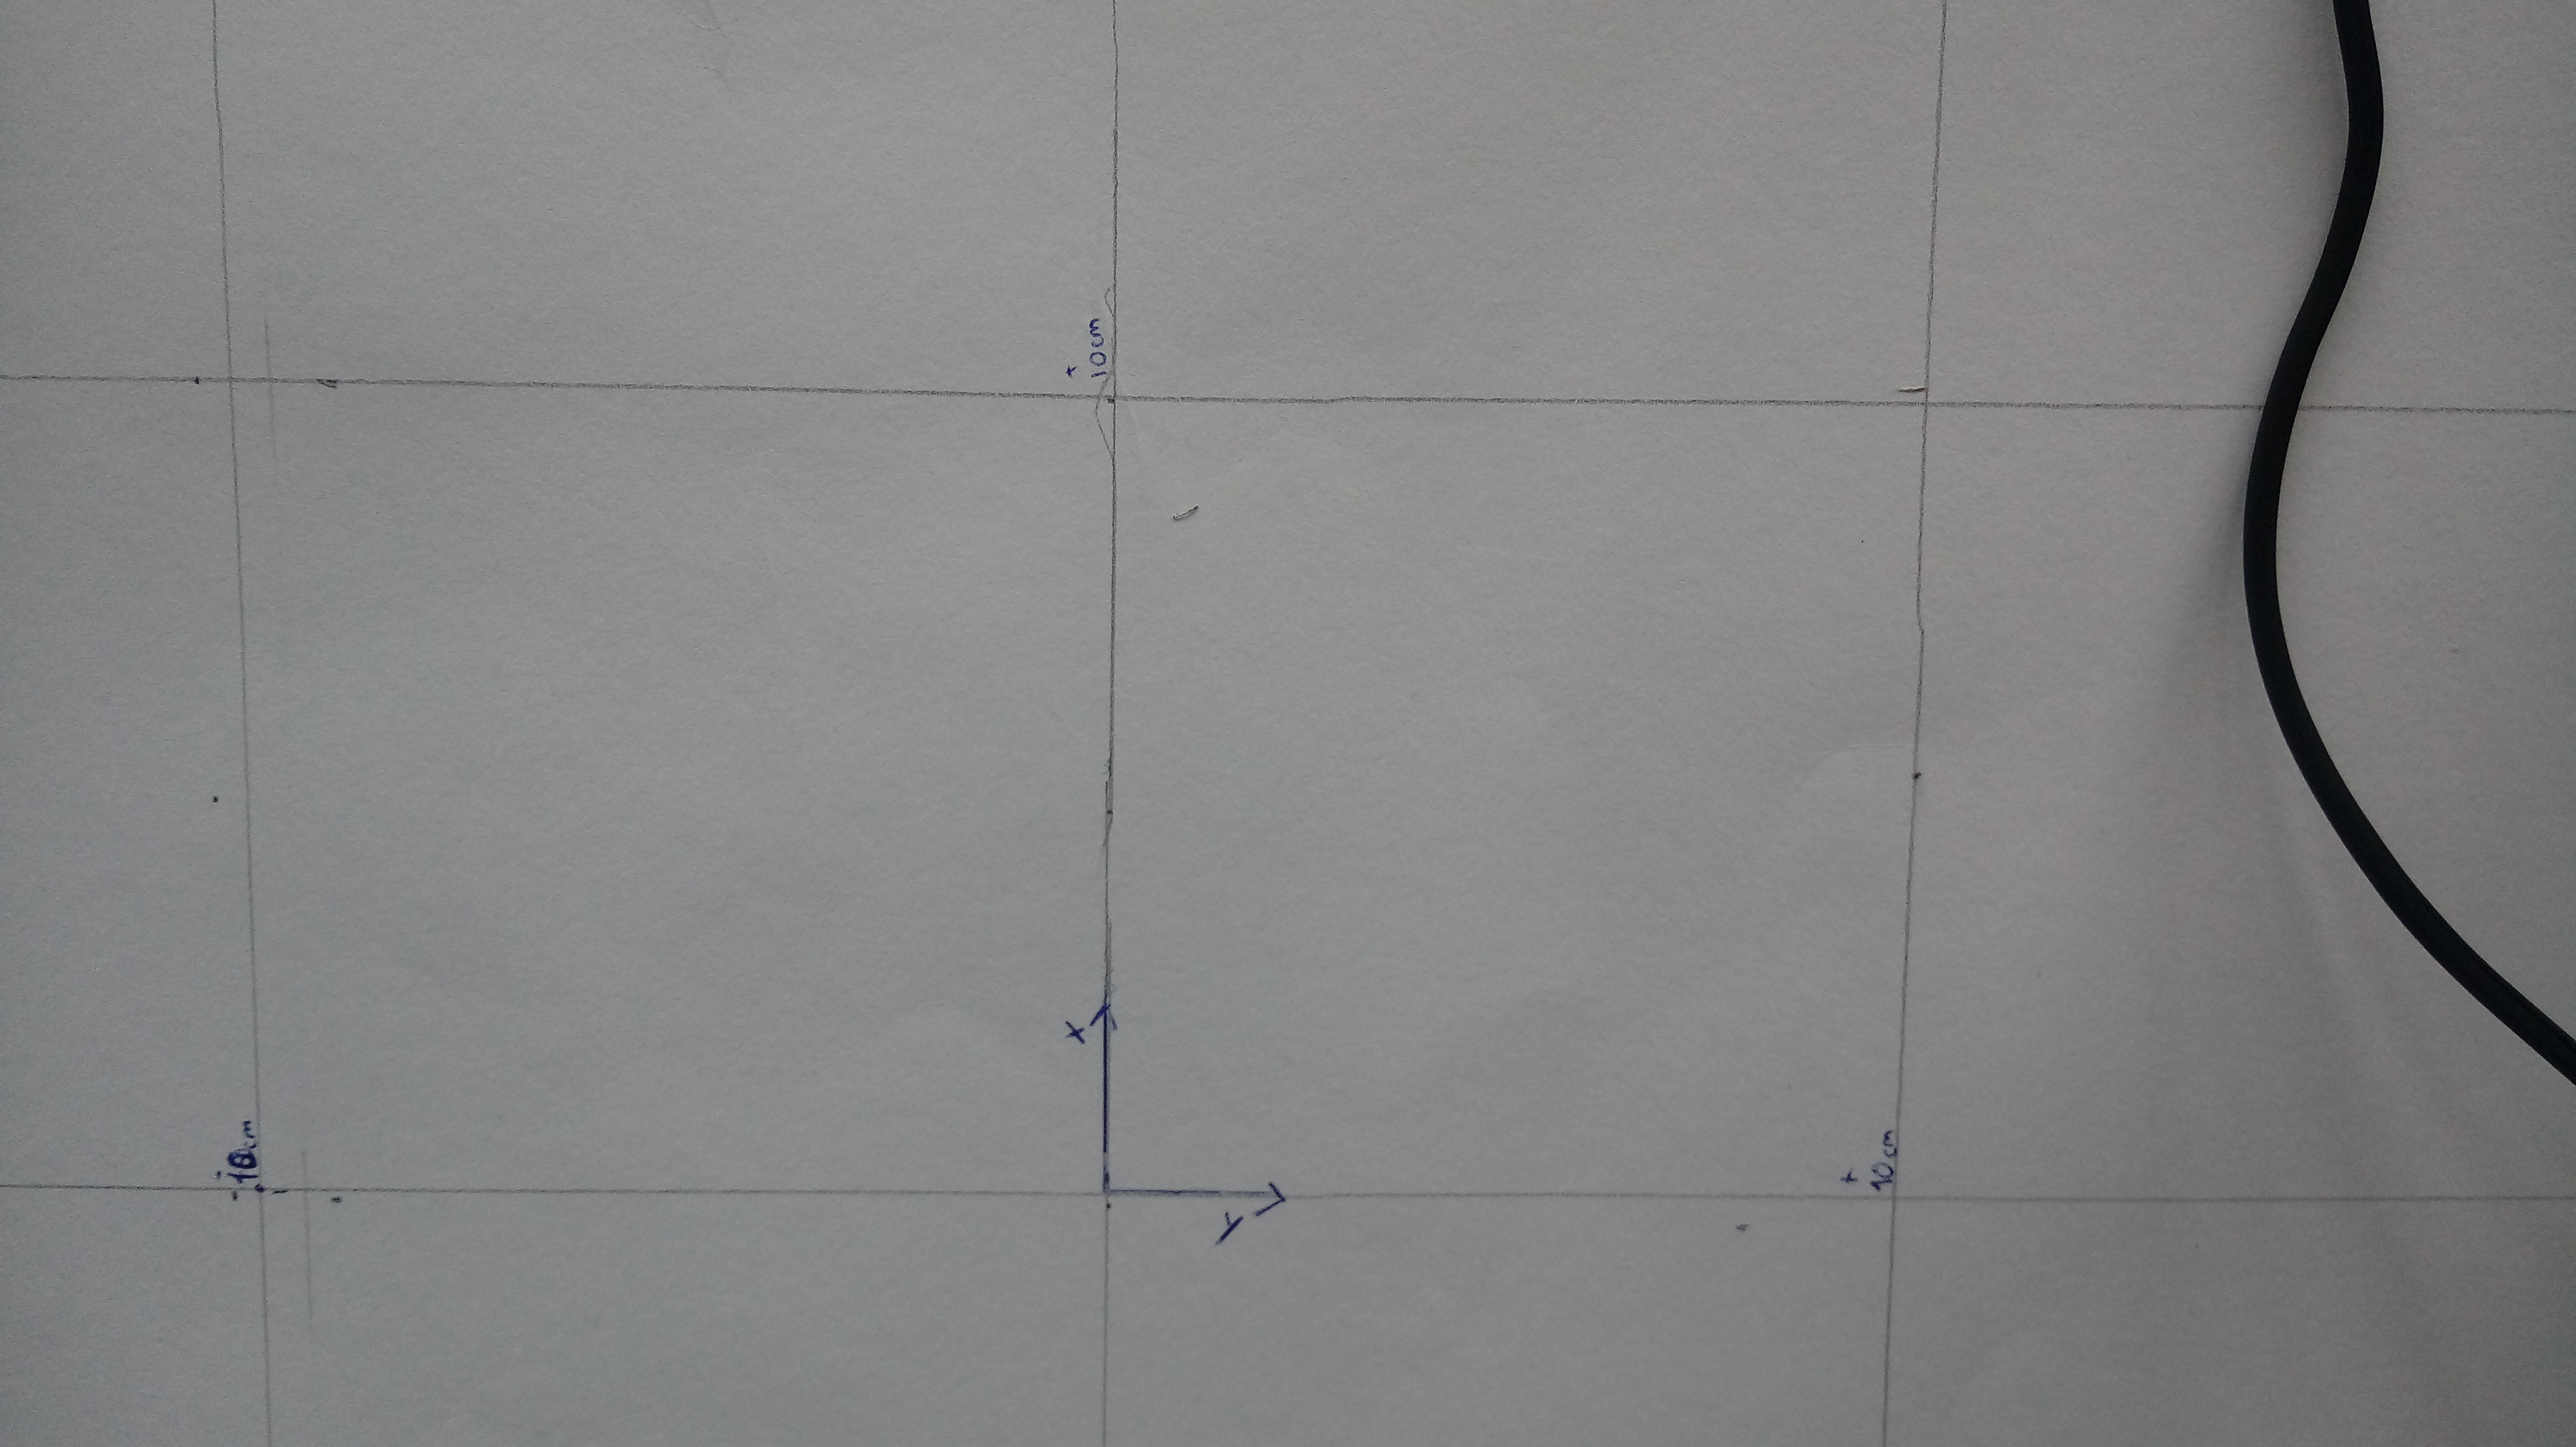
\includegraphics[trim=200 0 500 550,clip, scale=0.10]{images/settings4}
\caption{World Frame}
\label{fig:9}
\end{figure}

\subsection*{Data Processing}

The initial points from the sensors are shown at table \ref{tab:2}. Those set of points define the initial pose of the robot, as it is seen the robot angle is of  0 $^{\circ} $ from x axis.

\begin{table}[h!]
\caption{Origin Laser Sensor Points}
\label{tab:2}
\centering
\begin{tabular}{|c|c|c|}
\hline
\multicolumn{3}{|c|}{Initial Points}\\
\hline
\multicolumn{2}{|c|}{Frame}&World 	\\
\hline
&X&Y\\
\hline
Front Point&	12	&0\\
\hline
Back Point&	-8.7&0\\
\hline
\end{tabular}
\end{table}

We assume for this experiment that the robot center is in the middle of the robot therefore, the robot point center can be calculated as:

	\[
	x_wi = xb_i + \left(\frac{xf_i - xb_i}{2}\right)
	\]
	
	\[
	y_wi = yb_i + \left(\frac{yf_i - yb_i}{2}\right)
	\]

\small Where i is the number of the experiment, f are front points, b are back ones and 0 are initial points .\\

\normalsize
This step is important because origin point are not in the origin of the coordinate frame, therefore $x_i$ and $y_i$ must be translated .
	\[
	\theta = tan^{-1}\left(\frac{y_wi}{x_wi}\right)
	\]

\subsection*{Experiments Results}

The complete experiments results are at the attached file called $second\_see \_data\_.ods$.\\
\subsubsection*{Final Robot poses}

All measurements plot are shown at figure \ref{fig:10}. Remembering that parameters from the curves are symmetric we can see that the straight line is slightly deviated from the perpendicular axis.\\

\begin{figure}[H]
\caption{Robot stop position}
\label{fig:10}
\centering
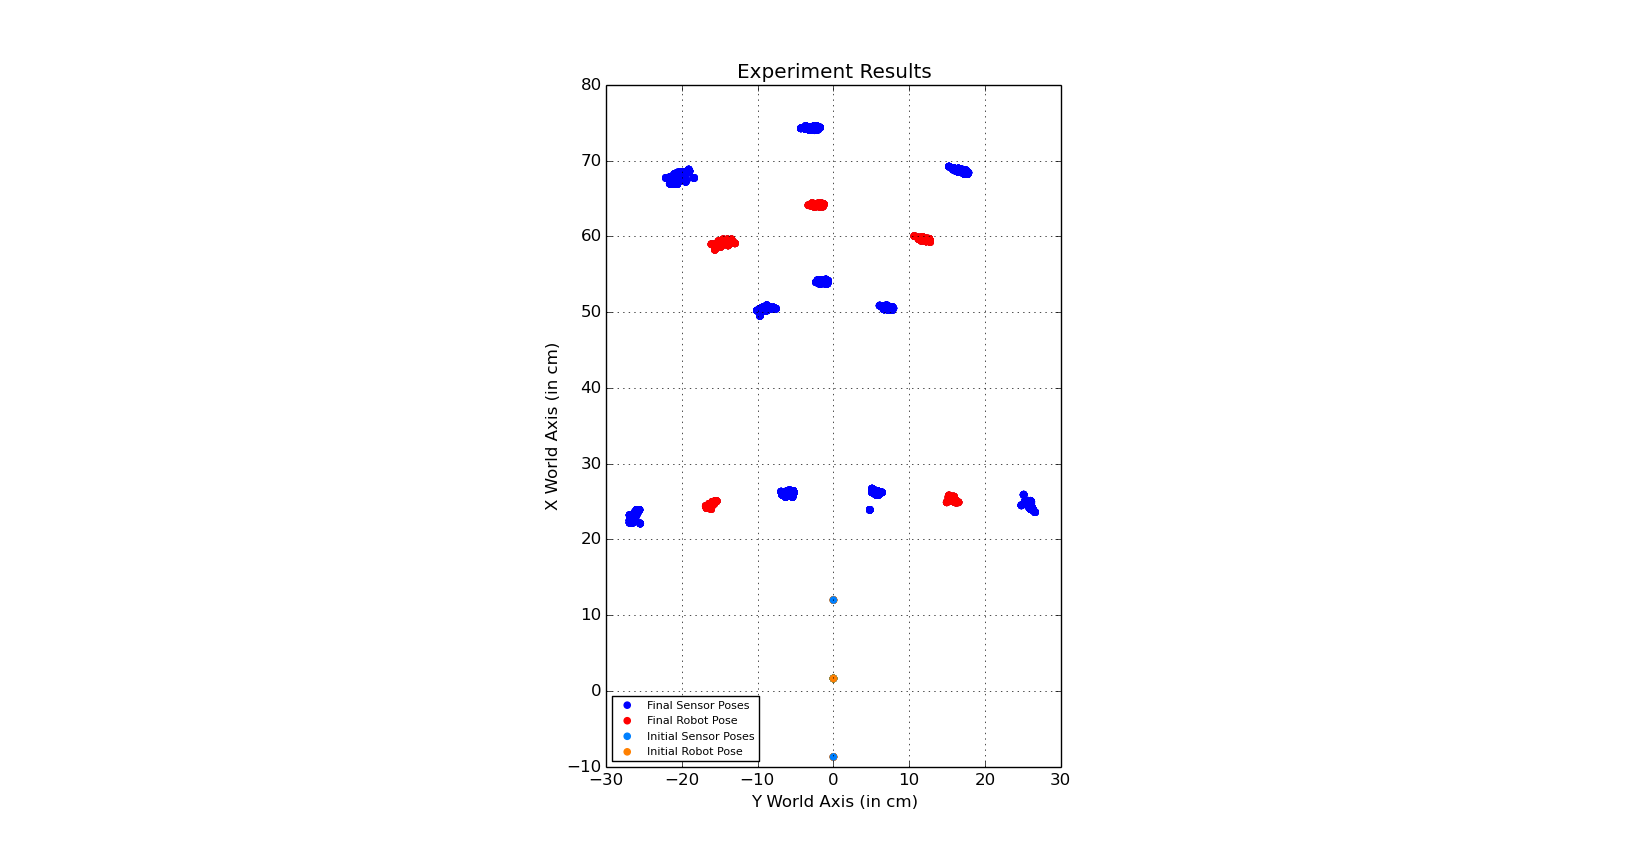
\includegraphics[trim={2000 0 2000 0},scale=0.70]{images/robot_pose_new_modified}
\end{figure}



\subsubsection*{Fitting Normal distribution to data}
\label{sec:fitdata}

The robot center poses were calculated and PCA was performed on these poses to find the principal components.The data was projected along the principal components and we tried to fit a gaussaian to the projected data.The results are depicetd below.


\begin{figure}[H]
\centering
\caption{Straight Line motion}
\label{fig:11}
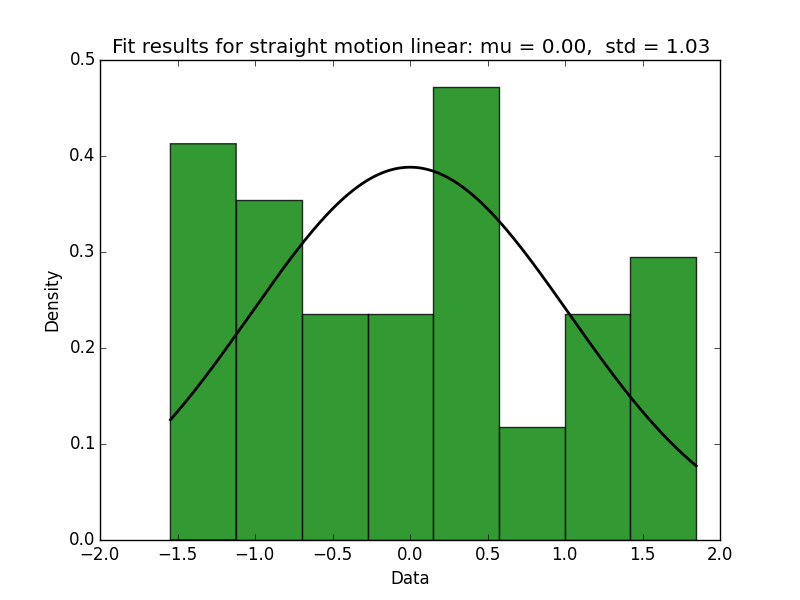
\includegraphics[width=0.49\textwidth ]{images/pca_straight_linear_data}
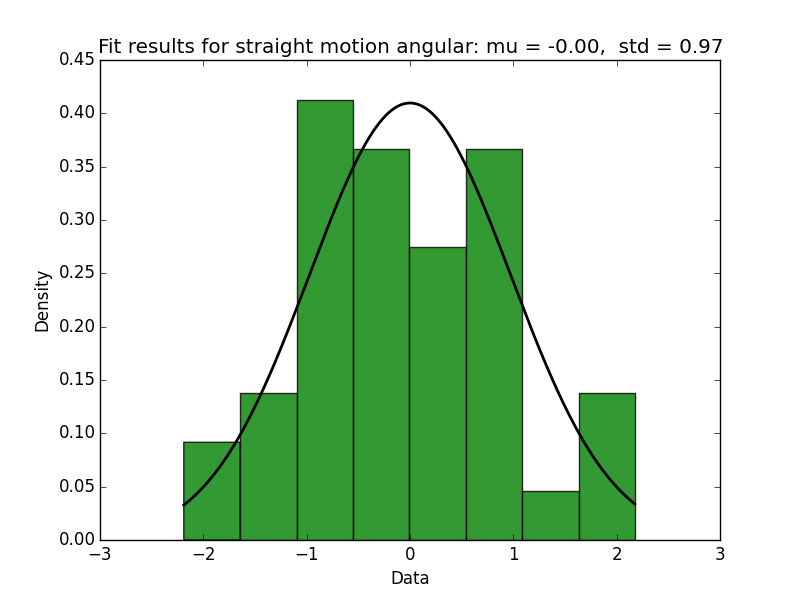
\includegraphics[width=0.49\textwidth]{images/pca_straight_angular_data}
\end{figure}

\begin{figure}[H]
\centering
\caption{Slight Right motion}
\label{fig:12}
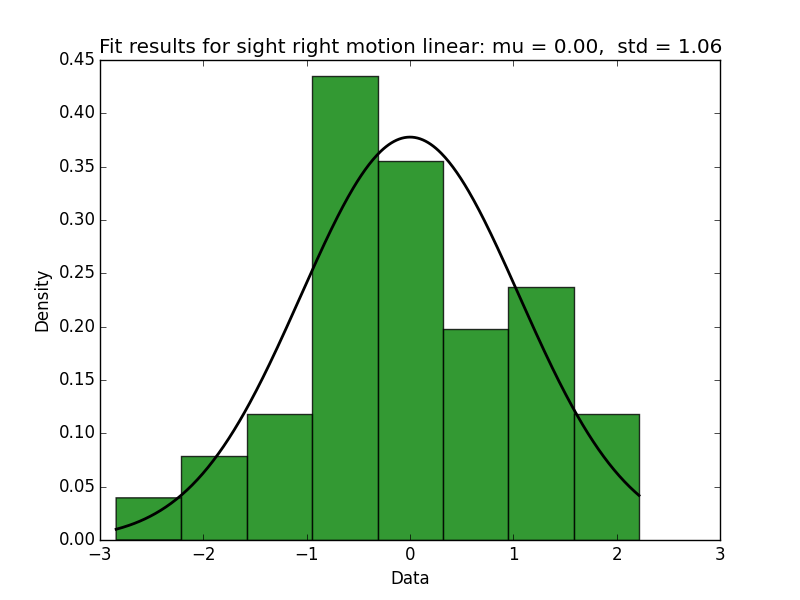
\includegraphics[width=0.49\textwidth ]{images/pca_slight_right_linear_data}
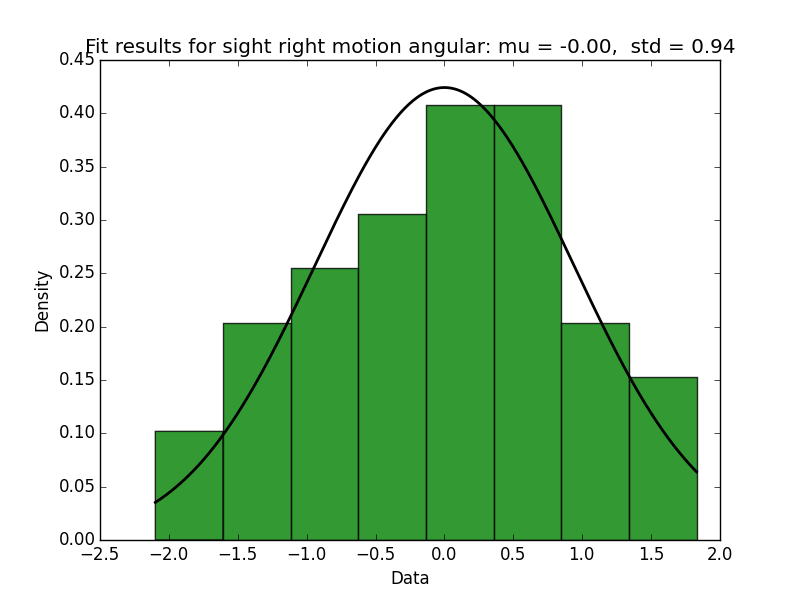
\includegraphics[width=0.49\textwidth]{images/pca_slight_right_angular_data}
\end{figure}

\begin{figure}[H]
\centering
\caption{Slight Left motion}
\label{fig:13}
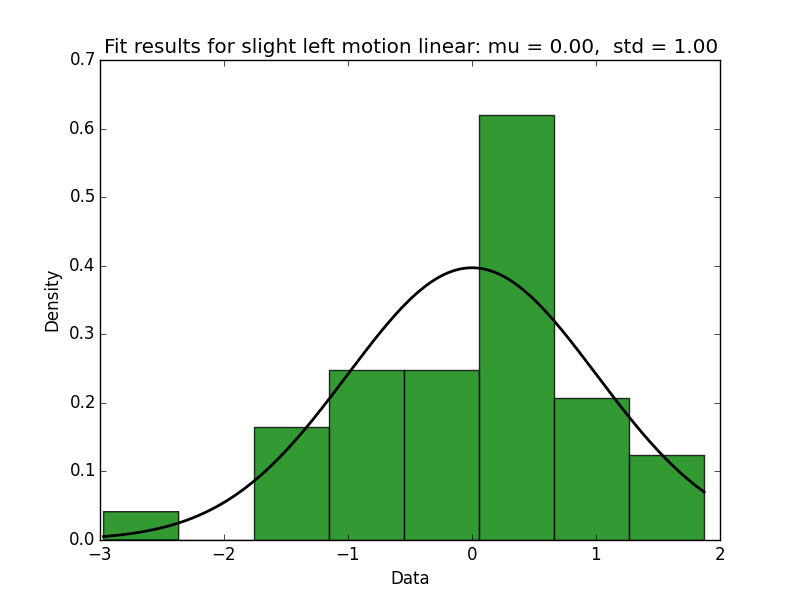
\includegraphics[width=0.49\textwidth ]{images/pca_slight_left_linear_data}
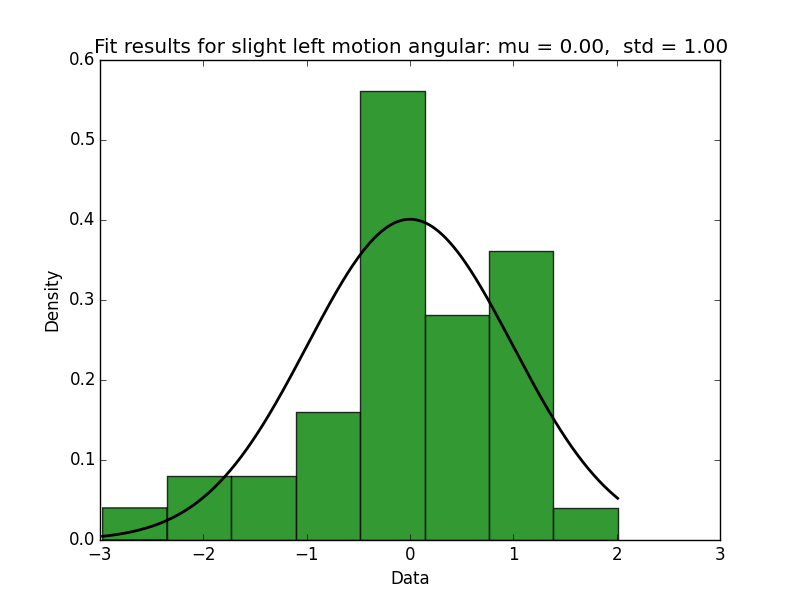
\includegraphics[width=0.49\textwidth]{images/pca_slight_left_angular_data}
\end{figure}

\begin{figure}[H]
\centering
\caption{Steep Right motion}
\label{fig:14}
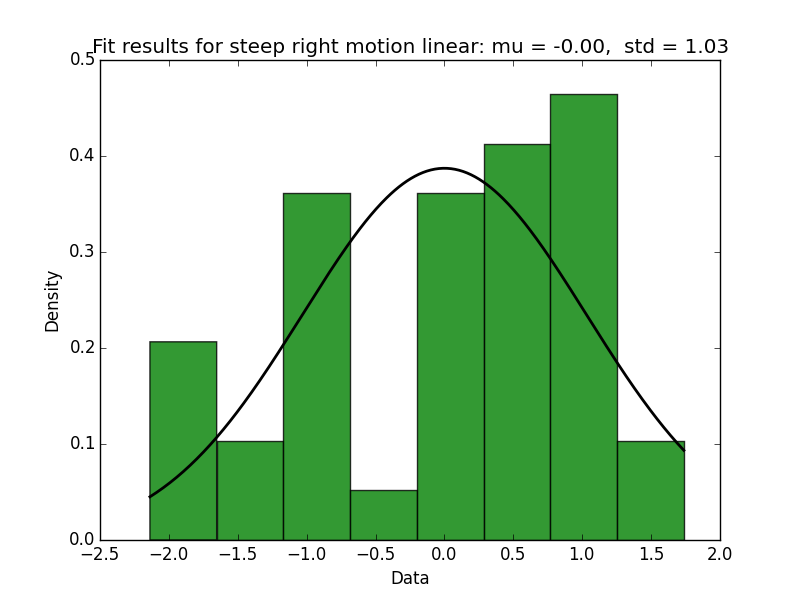
\includegraphics[width=0.49\textwidth ]{images/pca_steep_right_linear_data}
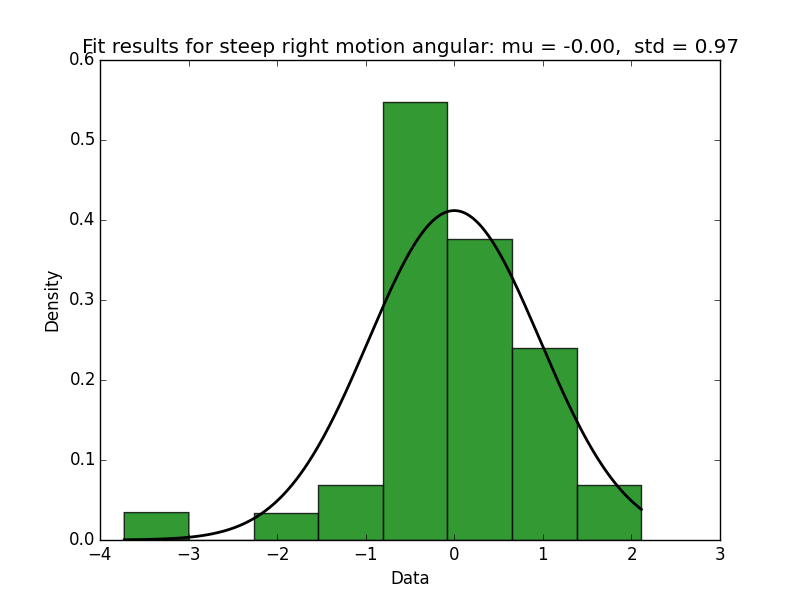
\includegraphics[width=0.49\textwidth]{images/pca_steep_right_angular_data}
\end{figure}

\begin{figure}[H]
\centering
\caption{Steep Left motion}
\label{fig:15}
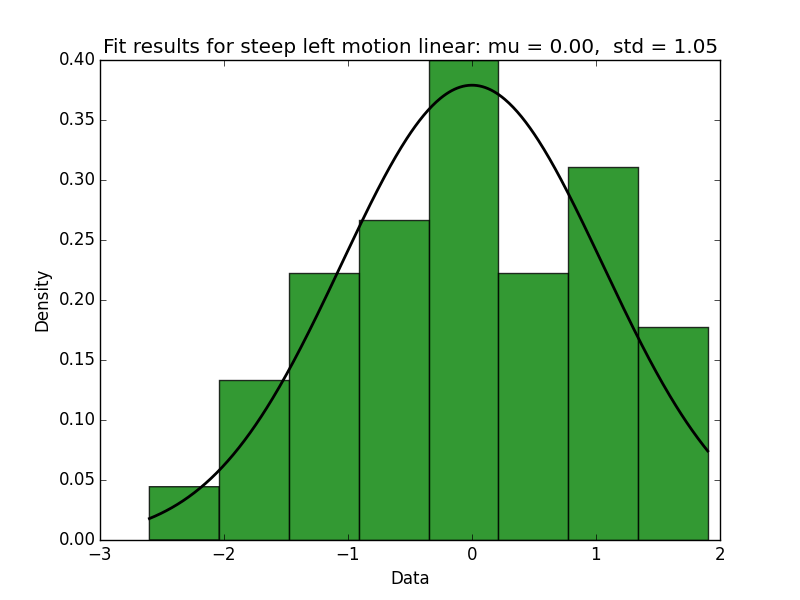
\includegraphics[width=0.49\textwidth ]{images/pca_steep_left_linear_data}
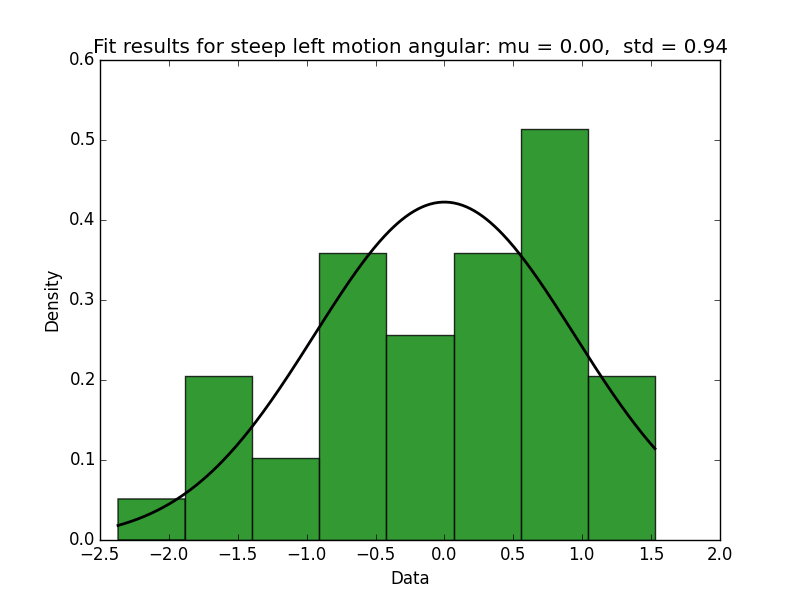
\includegraphics[width=0.49\textwidth]{images/pca_steep_left_angular_data}
\end{figure}

\section*{\hl{Conclusions}}

On the section \textit{"\nameref{sec:fitdata}"}, the Gaussian distribution of the measured poses were shown for the five curves. 

At each figure, the standard deviation were provided showing that the fit motion angular deviation is smaller or equal to the fit linear motion deviation. Also it can be appreciated that most of the measurements fit inside 2$\sigma$ gaussian distribution.

The last proofs that the error on the measurement fit on a $2\sigma$ Gaussian Distribution. This means that a $95\%$ of values will lie between the range $\left[-2\sigma,+2\sigma\right]$.

\end{document}